\documentclass[11pt]{article}
\usepackage{../EllioStyle}
\usepackage{fancyvrb}
\usepackage{pdfpages}
\usepackage{xcolor}


\usepackage{fancyvrb}

% redefine \VerbatimInput
\RecustomVerbatimCommand{\VerbatimInput}{VerbatimInput}%
{fontsize=\footnotesize,
 %
 frame=lines,  % top and bottom rule only
 framesep=2em, % separation between frame and text
 rulecolor=\color{gray},
 %
 label=\fbox{\color{black}design pattern finder output.txt},
 labelposition=topline,
 %
 commandchars=\|\(\), % escape character and argument delimiters for
                      % commands within the verbatim
 commentchar=*        % comment character
}


\title{Homework 6}
\author{Elliott Pryor}
\date{19 Nov 2020}


\begin{document}
\maketitle


\problem{1}
This system is designed to be as simple as possible. Working on the KISS principles. It prioritizes flexible methods for user interaction: web, mobile, or future technologies. 
The system is designed to interact with a variety of platforms in a comparable manner, giving users an equal experience regardless of platform.
It also prioritizes marketing allowing the business to create one uniform marketing strategy to roll out across all transactions.
The B2C and B2B interactions are self contained making it easier to change other components in the system (low coupling). 
It is built on one back-end system so that all processes can have high quality security and uniform record keeping. 

\begin{figure}[H]
    \centering
    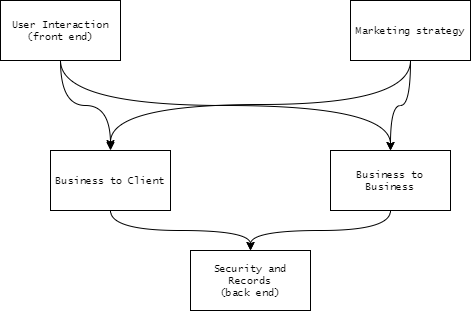
\includegraphics[scale = 0.7]{./p1_high_level.png}
    \caption{High Level diagram of the system}
    \label{fig:high level}
\end{figure}

\newpage
\problem{2}
\begin{figure}[H]
    \centering
    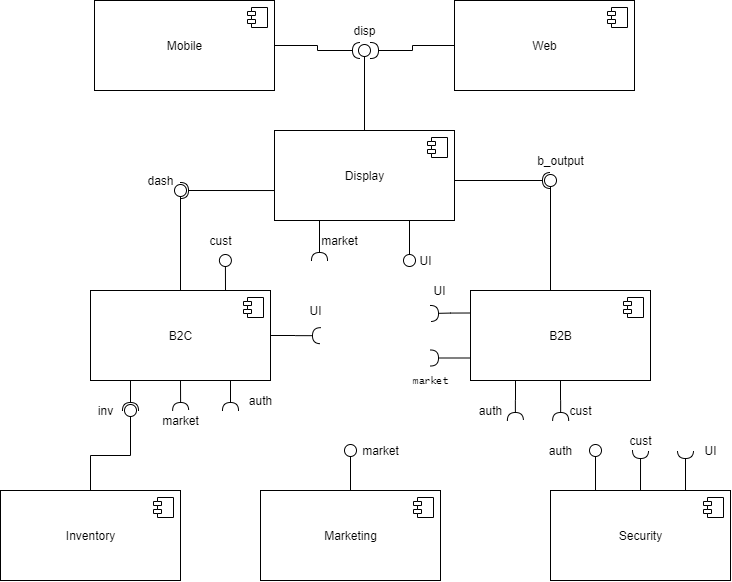
\includegraphics[width = \linewidth]{./p2_component.png}
    \caption{Component diagram}
    \label{fig:component}
\end{figure}

\newpage
\problem{3}

This takes user inputs in and manages them with the Organization method. The organization method can lookup user credentials and find the proper user. Then it can apply changes made in the UI of choice (web/mobile) to the customer object. Like add a searched object in to a wishlist, or connect a new social media account. The social media accounts use the strategy pattern to allow connecting many accounts. It is also easy to expand the business and add a new account type. 

\begin{figure}[H]
    \centering
    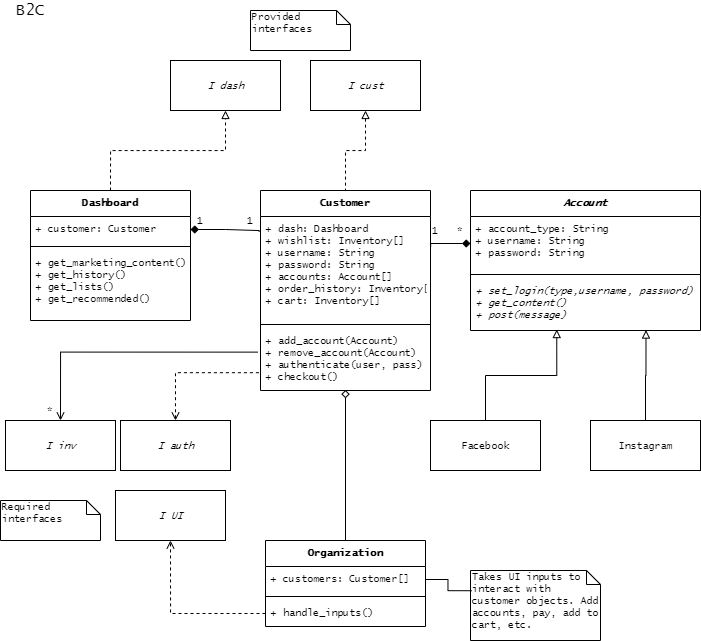
\includegraphics[width = \linewidth]{./p3_uml.png}
    \caption{UML Diagram of B2C component}
    \label{fig:uml}
\end{figure}

\end{document}